\section{核反应堆控制系统的稳定性分析}

请先自行复习《自动控制原理》中闭环特征方程式、根轨迹、奈奎斯特图及判据的相关知识,本章的题目大多是在上学期自控题目的基础上引入了核反应堆控制的背景,会解答具体题目,了解不同类型核反应堆系统的稳定性结论即可应对考试。

\subsection{核反应堆系统稳定性}

根轨迹始终在左半$s$平面,则核反应堆系统稳定。

\subsubsection{两路并联温度反馈}

\begin{enumerate}
    \item $H_{\rm f} + H_{\rm s} > 0$时,系统必不稳定(反馈为正);
    \item $H_{\rm f} + H_{\rm s} < 0$时,系统不一定稳定。
\end{enumerate}

\subsubsection{两路串联温度反馈}

\begin{enumerate}
    \item $\alpha_{\rm f} + \alpha_{\rm m} > 0$,系统必不稳定;
    \item $\alpha_{\rm f} + \alpha_{\rm m} < 0$,系统不一定稳定;
    \item $\alpha_{\rm f}$的效应更快更强。
\end{enumerate}

\subsubsection{石墨气冷动力堆}

反应性慢化剂温度系数上限是
\begin{equation}
    \alpha_{\rm mc} = -\alpha_{\rm f}\frac{K_{\rm fA}}{K_{\rm fB}}
\end{equation}

\begin{enumerate}
    \item 运行初期,$\alpha_{\rm f} < 0$,$\alpha_{\rm m} < 0$,随着燃耗加深,逐渐过渡为$\alpha_{\rm f} < 0$,$\alpha_{\rm m} > 0$;
    \item $\alpha_{\rm m} < \alpha_{\rm mc}$时,系统稳定;$\alpha_{\rm m} > \alpha_{\rm mc}$时,系统不稳定;
    \item 正常运行时,石墨堆天然满足$\alpha_{\rm m} > \alpha_{\rm mc}$,即石墨堆固有不稳定,即使将气体出口温度效应考虑进来也无法改变。
\end{enumerate}

\subsection{实验研究型核反应堆}

需要复习《自动控制原理》中关于降阶简化特征方程的相关知识。

\begin{enumerate}
    \item 重水堆的减速器传递系数$K > 2.064$时,系统不稳定;$K < 2.064$时,系统稳定;
    \item 实验研究堆固有稳定。
\end{enumerate}

\subsection{动力堆稳定性}

动力堆带有位置反馈(控制棒),提高了系统稳定性(稳定域扩大一倍),改善了系统的控制性能(瞬态响应更好)。

动力堆稳定的必要条件是其位置反馈传递系数$K_{\rm f} < K_{\rm fc} = |OA|$,调节动力堆系统稳定性,就是要调节系数$K_C$,使得奈奎斯特图中的$(-1,\,j0)$点落在使系统稳定的范围内。

\subsection{数字控制系统稳定性}

请先自行复习劳斯判据的相关知识,特别是不要忘记其必要条件(闭环特征方程不缺项)。

\begin{figure}[H]
    \centering
    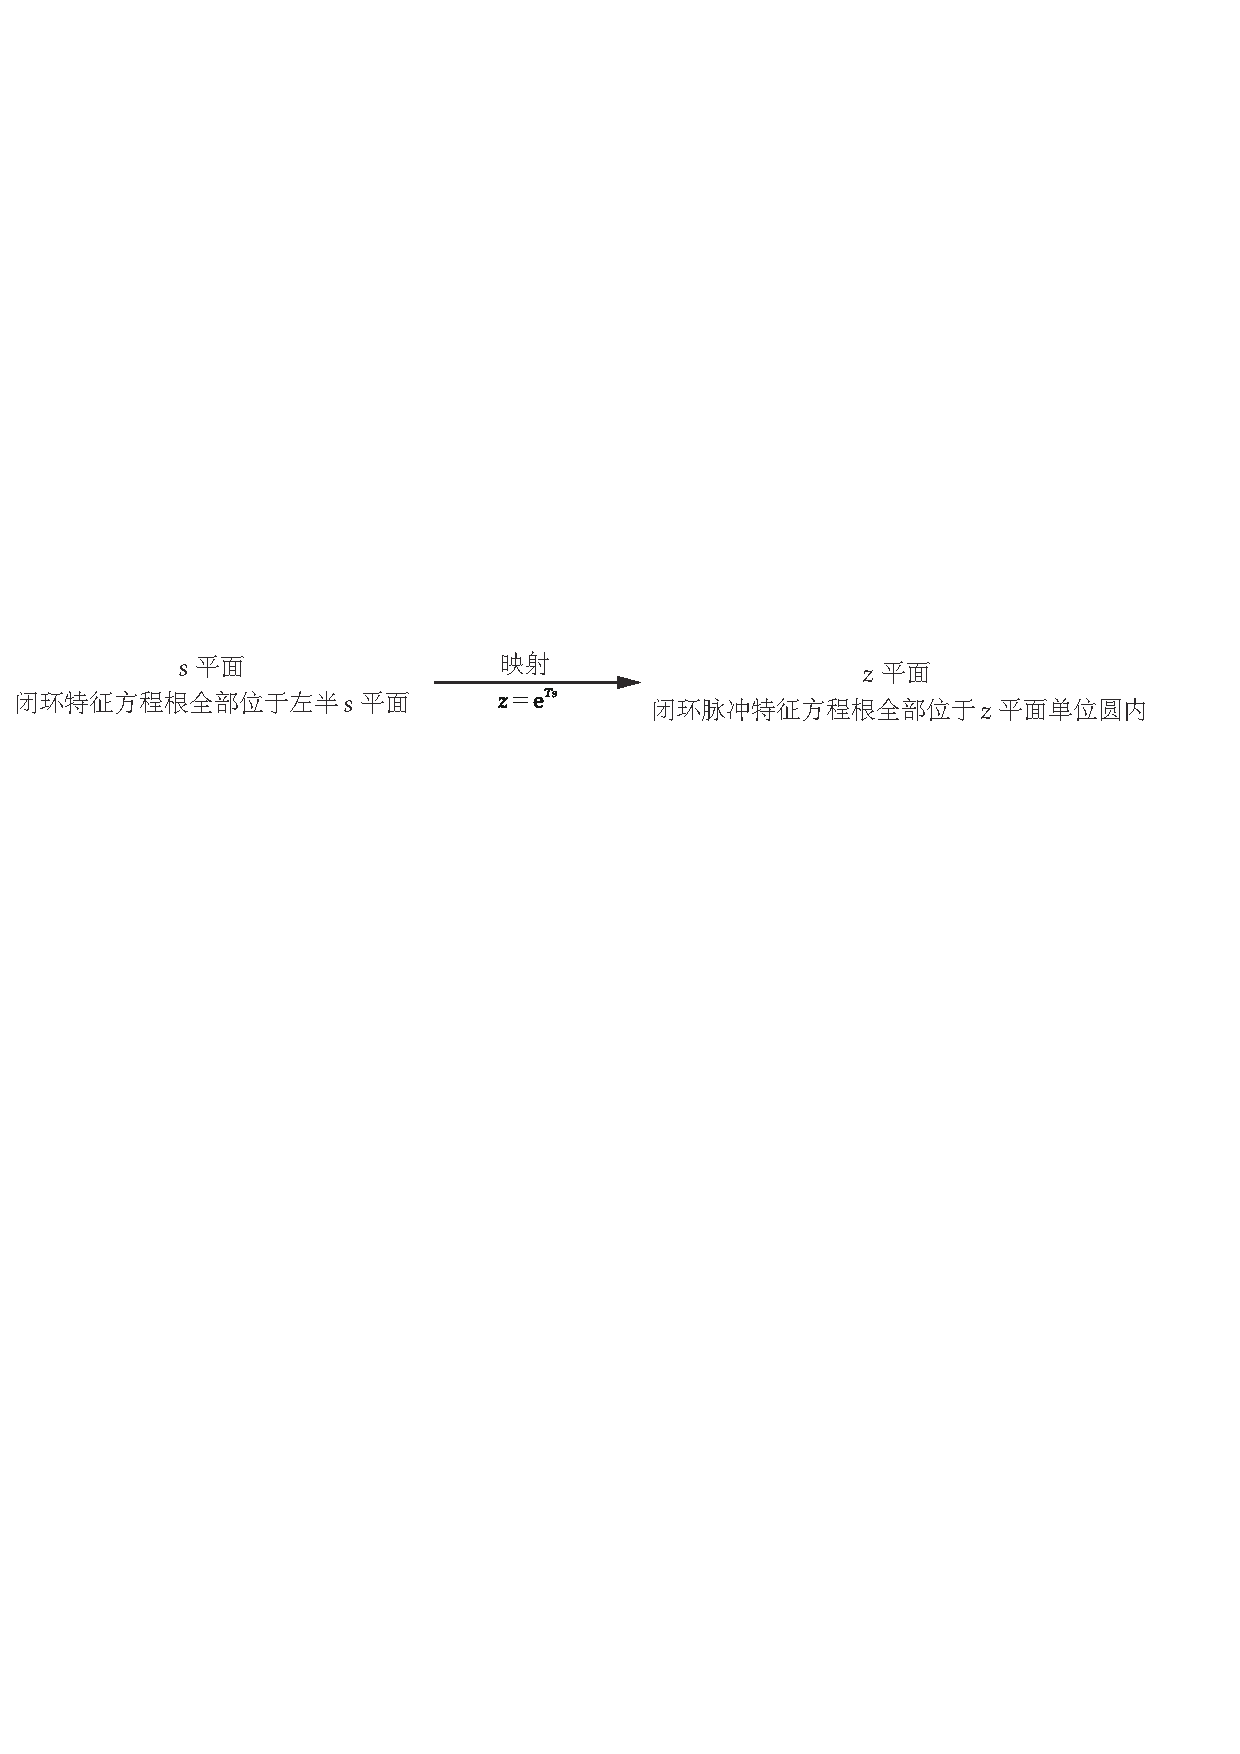
\includegraphics[scale=0.7]{figures/figure5.1.pdf}
\end{figure}

朱利判据了解即可,这里给出两种稳定性判据。

\begin{enumerate}
    \item 直接对闭环脉冲特征方程求解,观察其是否位于$z$平面单位圆内;
    \item 令$w = \frac{z+1}{z-1}$,从$z$平面映射到$w$平面,再使用劳斯判据。
\end{enumerate}

\subsection{核反应堆稳定性状态空间分析}

这里补充实对称矩阵正、负定的判断,具体解题过程参照习题选解。
\begin{enumerate}
    \item 某实对称矩阵$\symbfit{P}$正定 $\Leftrightarrow$ $\symbfit{P}$的所有主子行列式均为正;
    \item 某实对称矩阵$\symbfit{P}$负定 $\Leftrightarrow$ $\symbfit{P}$的奇主子行列式均为负,偶主子行列式均为正。
\end{enumerate}

\subsection{习题选解}

\begin{exercise} % 5.1
    \begin{enumerate}
        \item 令$s=j\varomega$,得
        \begin{align*}
            G(j\varomega)H(j\varomega) &= \frac{K(1-\varomega^2)}{1+\varomega^2} - j\frac{2K\varomega}{1+\varomega^2} \\
            {\rm Re}(\varomega) &= \frac{K(1-\varomega^2)}{1+\varomega^2} \\
            {\rm Im}(\varomega) &= -\frac{2K\varomega}{1+\varomega^2}
        \end{align*}
        \item 起始点,$\varomega \to 0^+$,${\rm Re}(0^+) = K$,${\rm Im}(0^+) = 0^-$;
        终止点,$\varomega \to +\infty$,${\rm Re}(+\infty) = -K$,${\rm Im}(+\infty) = -\infty$
        \item 象限
        \begin{table}[H]
            \centering
            \begin{tabular}{ccc}
                \toprule
                $\varomega$ & $0^+$ & $+\infty$ \\
                \hline
                $K$ & $0^{\circ}$ & $0^{\circ}$ \\
                $1-s$ & $0^{\circ}$ & $-90^{\circ}$ \\
                $\frac{1}{s+1}$ & $0^{\circ}$ & $-90^{\circ}$ \\
                \hline
                $\varphi(\varomega)$ & $0^{\circ}$ & $-180^{\circ}$ \\
                \bottomrule
            \end{tabular}
        \end{table}
        \item 与坐标轴交点
        \begin{enumerate}
            \item ${\rm Im}(\varomega)=0$,$\varomega = 0$(或$\infty$),${\rm Re}(0) = \pm K$,即交点为$(\pm K,\,0)$;
            \item ${\rm Re}(\varomega)=0$,$\varomega = \pm 1$,${\rm Im}(\pm 1) = \mp K$,即交点为$(0,\,\mp K)$。
        \end{enumerate}
        无开环右极点,奈奎斯特图如下。
        \begin{figure}[H]
            \centering
            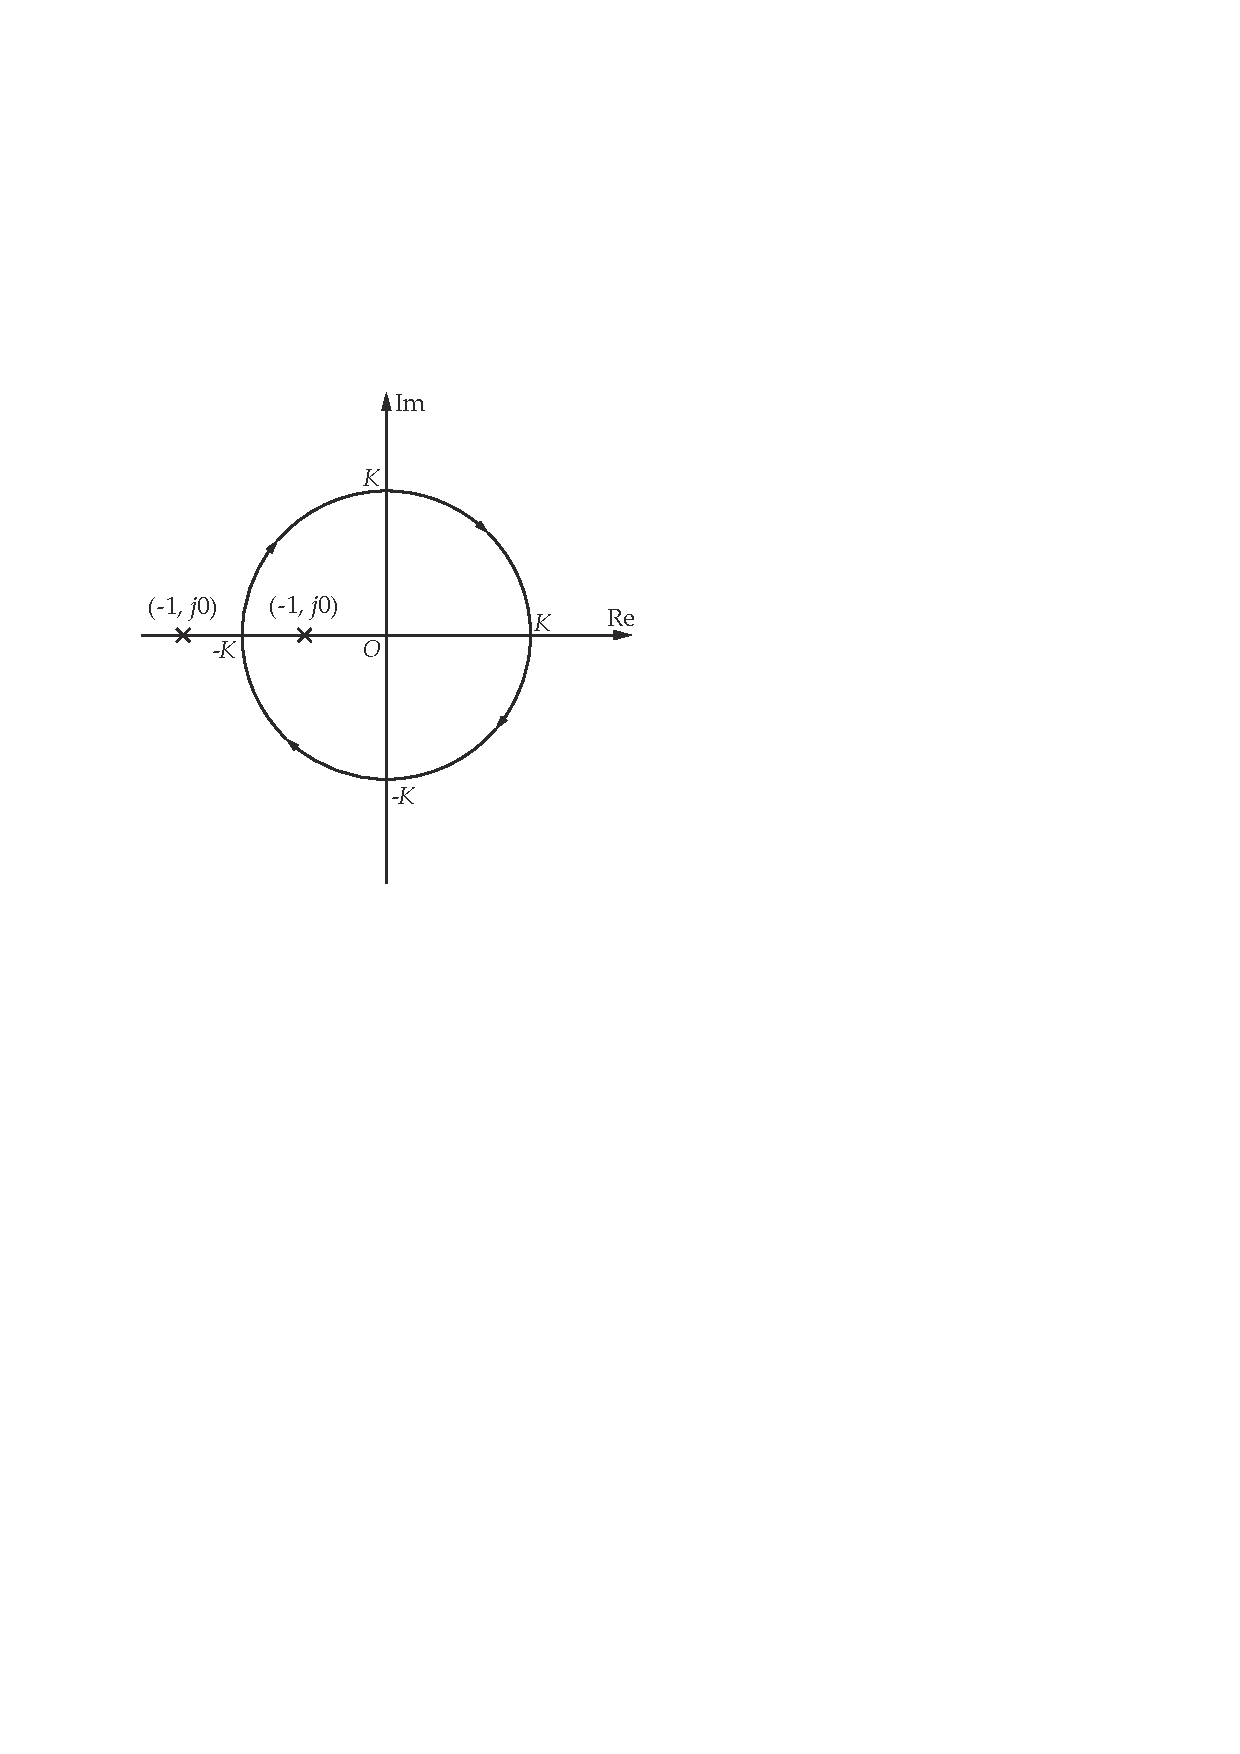
\includegraphics[scale=0.6]{figures/figure5.2.pdf}
        \end{figure}
    \end{enumerate}
    \begin{enumerate}
        \item 若$K<1$,奈奎斯特轨迹不包围$(-1,\,j0)$点,系统闭环稳定;
        \item 若$K\geqslant 1$,奈奎斯特轨迹包围(或经过)$(-1,\,j0)$点,系统闭环不稳定。
    \end{enumerate}
\end{exercise}

\begin{exercise} % 5.2
    \begin{enumerate}
        \item $z_1 = 0.5+0.6181i$,$z_2 = 0.5-0.6181i$,均在$z$平面单位圆内,系统稳定;
        \item $z_1 = -0.5123$,$z_2 = 1.487$,$z_3 = 0.5250$,$z_2$不在$z$平面单位圆内,系统不稳定;
        \item $z_1 = 0.5$,$z_2 = 0.5+0.5i$,$z_3 = 0.5-0.5i$,均在$z$平面单位圆内,系统稳定。
    \end{enumerate}
    或使用劳斯判据。
\end{exercise}

\begin{exercise} % 5.3
    \begin{align*}
        G(z) &= \Z{\frac{1-{\rm e}^{Ts}}{s} \cdot \frac{1}{s(s+1)}} = (1-z^{-1})\left[\frac{1}{s^2(s+1)}\right] \\
        &= (1-z^{-1})\Z{\frac{1}{s^2} - \frac{1}{s} + \frac{1}{s+1}} = (1-z^{-1})\left[\frac{zT}{(z-1)^2} - \frac{z}{z-1} + \frac{z}{z-{\rm e}^{-T}}\right] \\
        &= \frac{zT(z-{\rm e}^{-T})-z(z-1)(z-{\rm e}^{-T})+z(z-1)^2}{z(z-1)(z-{\rm e}^{-T})}
    \end{align*}
    由题意,$T=1\,{\rm s}$,则
    \begin{equation*}
        G(z) = \frac{0.3679z + 0.2642}{z^2-1.3679z+0.3679}
    \end{equation*}
    闭环特征方程$D(z) = z^2 - z + 0.6321$,解得$z=0.5 \pm 0.6181j$,均在$z$平面单位圆内,系统稳定。
\end{exercise}

\setcounter{exercise}{7}

\begin{exercise} % 5.8
    \begin{enumerate}
        \item $\gamma = 0.01\,{\rm s}^{-1}$时,$K_{\rm R}G_{\rm R}(s)H(s) = \frac{K(s+0.1)}{s(s+0.01)(s+100)}$
        \begin{enumerate}
            \item 起始点:$z_1 = 0$,$z_2 = -0.01$,$z_3 = -100$;
            终止点:$p_1 = -0.1$;
            \item 实轴上的根轨迹:$[-100,\,-0.1]$,$[-0.01,\,0]$;
            \item 分支数为3,两支终止于无穷远处;
            \item 渐近线
            \begin{align*}
                -\sigma_a &= -\frac{-0.1-(0-0.01-100)}{3-1} = -49.955 \\
                \theta_k &= \frac{\pm (2k+1)\pi}{3-1} = \begin{cases}
                    \pm \frac{\pi}{2},\,k=0 \\
                    \pm \frac{3\pi}{2},\,k=1
                \end{cases}
            \end{align*}
            \item 分离点与会合点
            闭环特征方程$s(s+0.01)(s+100)+K(s+0.1) = 0$,于是有
            \begin{equation*}
                K = -\frac{s(s+0.01)(s+100)}{s+0.1}
            \end{equation*}
            令$\dv{K}{s} = 0$,得
            \begin{equation*}
                2s^3 + 100.31s^2 + 20.002s + 0.1 = 0 \Rightarrow \begin{cases}
                    s_1 = -49.955 \\
                    s_2 = -0.00513 \\
                    s_3 = -0.195
                \end{cases}
            \end{equation*}
            其中,$s_1$和$s_2$为分离点,$s_3$为会合点。
            \item 与虚轴的交点
            闭环特征方程中令$s=-j\varomega$,得
            \begin{equation*}
                -j\varomega^3 - 100.01\varomega^2 + (1+K)j\varomega + 0.1K = 0 \Rightarrow \begin{cases}
                    \varomega^3 - (1+K) \varomega = 0 \\
                    100.01\varomega^2 - 0.1K = 0
                \end{cases} \Rightarrow \begin{cases}
                    K = 0 \\
                    \varomega = 0
                \end{cases}
            \end{equation*}
            只与原点相交。
        \end{enumerate}
        故,根轨迹如下。
        \begin{figure}[H]
            \centering
            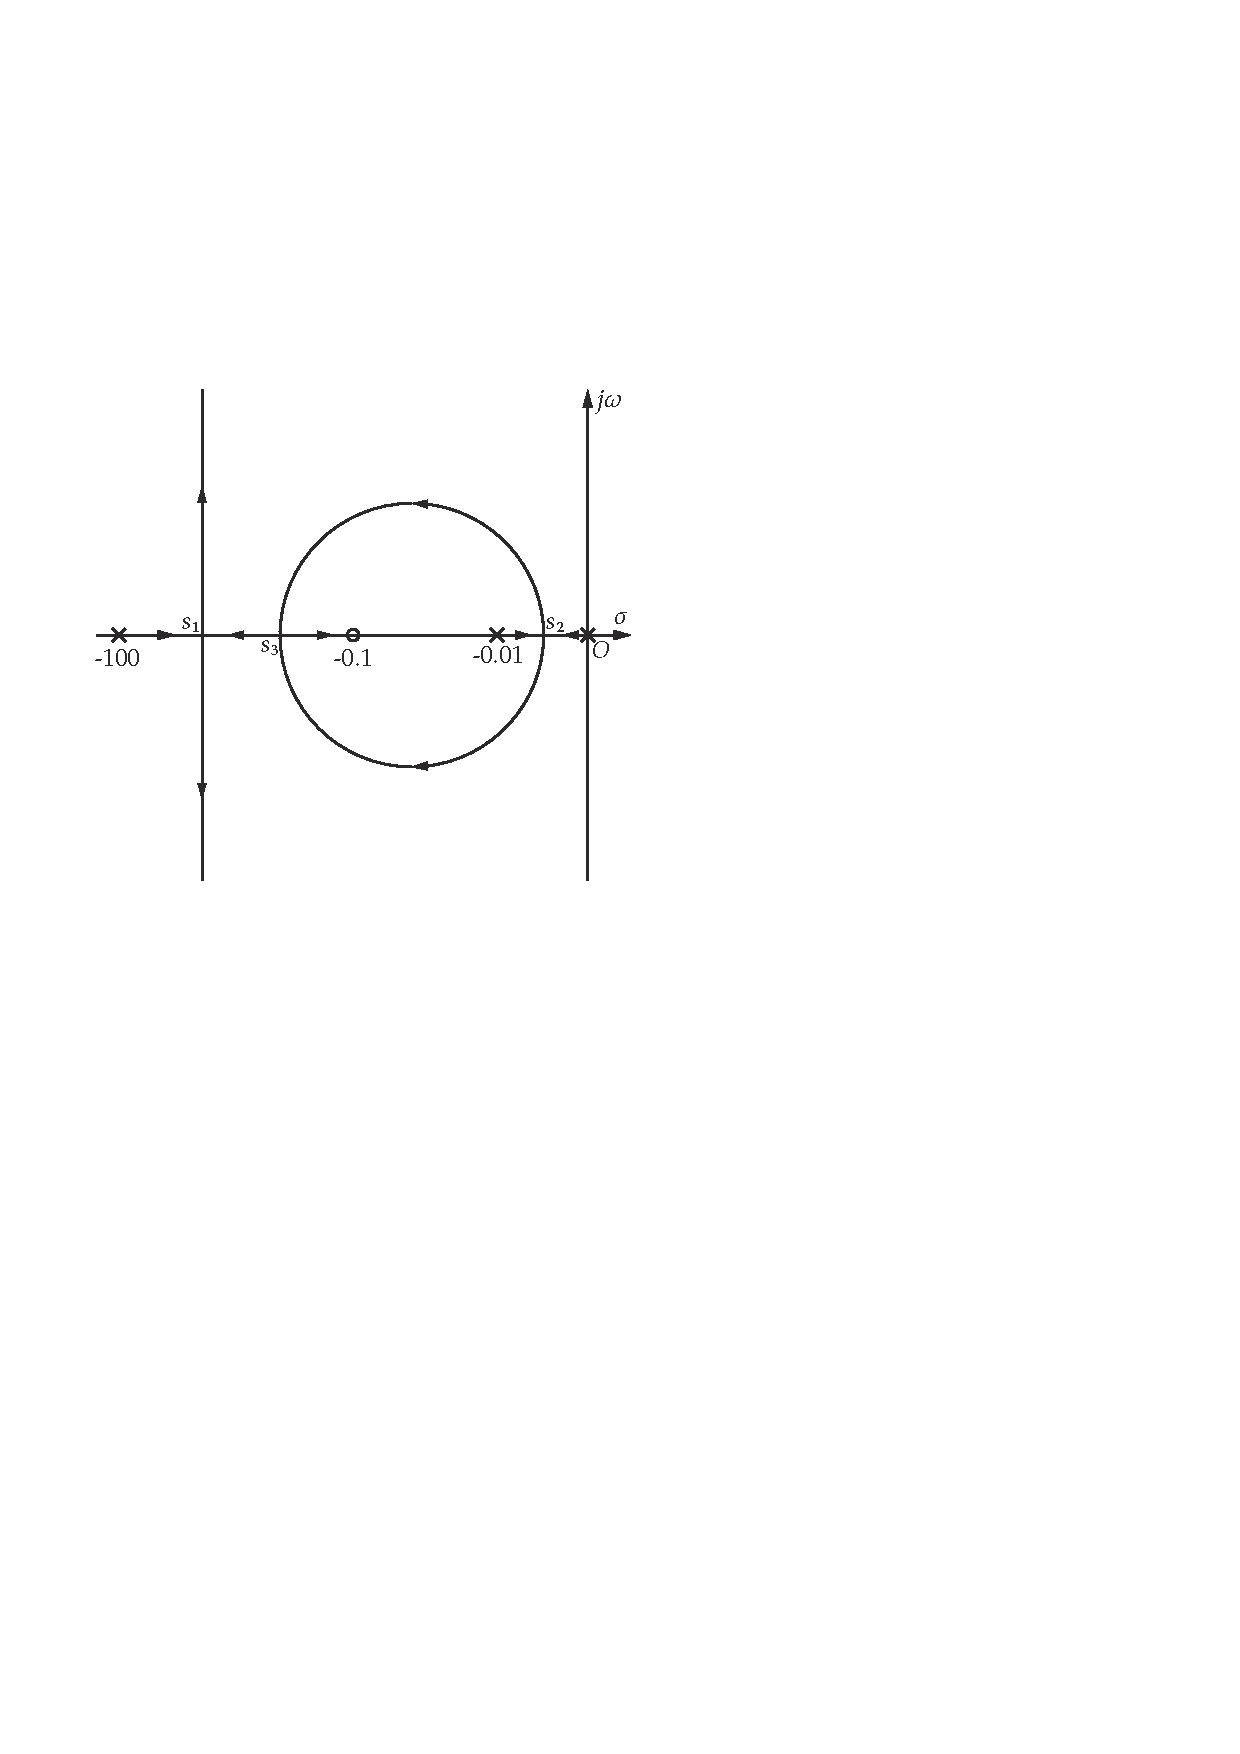
\includegraphics[scale=0.6]{figures/figure5.3.pdf}
        \end{figure}
        \item $\gamma = 1\,{\rm s}^{-1}$时,$K_{\rm R}G_{\rm R}(s)H(s) = \frac{K(s+0.1)}{s(s+1)(s+100)}$
        \begin{enumerate}
            \item 起始点:$z_1 = 0$,$z_2 = -1$,$z_3 = -100$;
            终止点:$p_1 = -0.1$;
            \item 实轴上的根轨迹:$[-100,\,-1]$,$[-0.1,\,0]$;
            \item 分支数为3,两支终止于无穷远处;
            \item 渐近线
            \begin{align*}
                -\sigma_a &= -\frac{-0.1-(0-1-100)}{3-1} = -50.45 \\
                \theta_k &= \frac{\pm (2k+1)\pi}{3-1} = \begin{cases}
                    \pm \frac{\pi}{2},\,k=0 \\
                    \pm \frac{3\pi}{2},\,k=1
                \end{cases}
            \end{align*}
            \item 分离点与会合点
            闭环特征方程$s(s+1)(s+100)+K(s+0.1) = 0$,于是有
            \begin{equation*}
                K = -\frac{s(s+1)(s+100)}{s+0.1}
            \end{equation*}
            令$\dv{K}{s} = 0$,得
            \begin{equation*}
                2s^3 + 101.3s^2 + 20.2s + 10 = 0 \Rightarrow \begin{cases}
                    s_1 = -50.45 \\
                    s_{2,3} = -0.1 \pm 0.3j
                \end{cases}
            \end{equation*}
            其中,$s_1$为分离点。
            \item 与虚轴的交点
            闭环特征方程中令$s=-j\varomega$,得
            \begin{equation*}
                -j\varomega^3 - 101\varomega^2 + (100+K)j\varomega + 0.1K = 0 \Rightarrow \begin{cases}
                    \varomega^3 - (100+K) \varomega = 0 \\
                    101\varomega^2 - 0.1K = 0
                \end{cases} \Rightarrow \begin{cases}
                    K = 0 \\
                    \varomega = 0
                \end{cases}
            \end{equation*}
            只与原点相交。
        \end{enumerate}
        故,根轨迹如下。
        \begin{figure}[H]
            \centering
            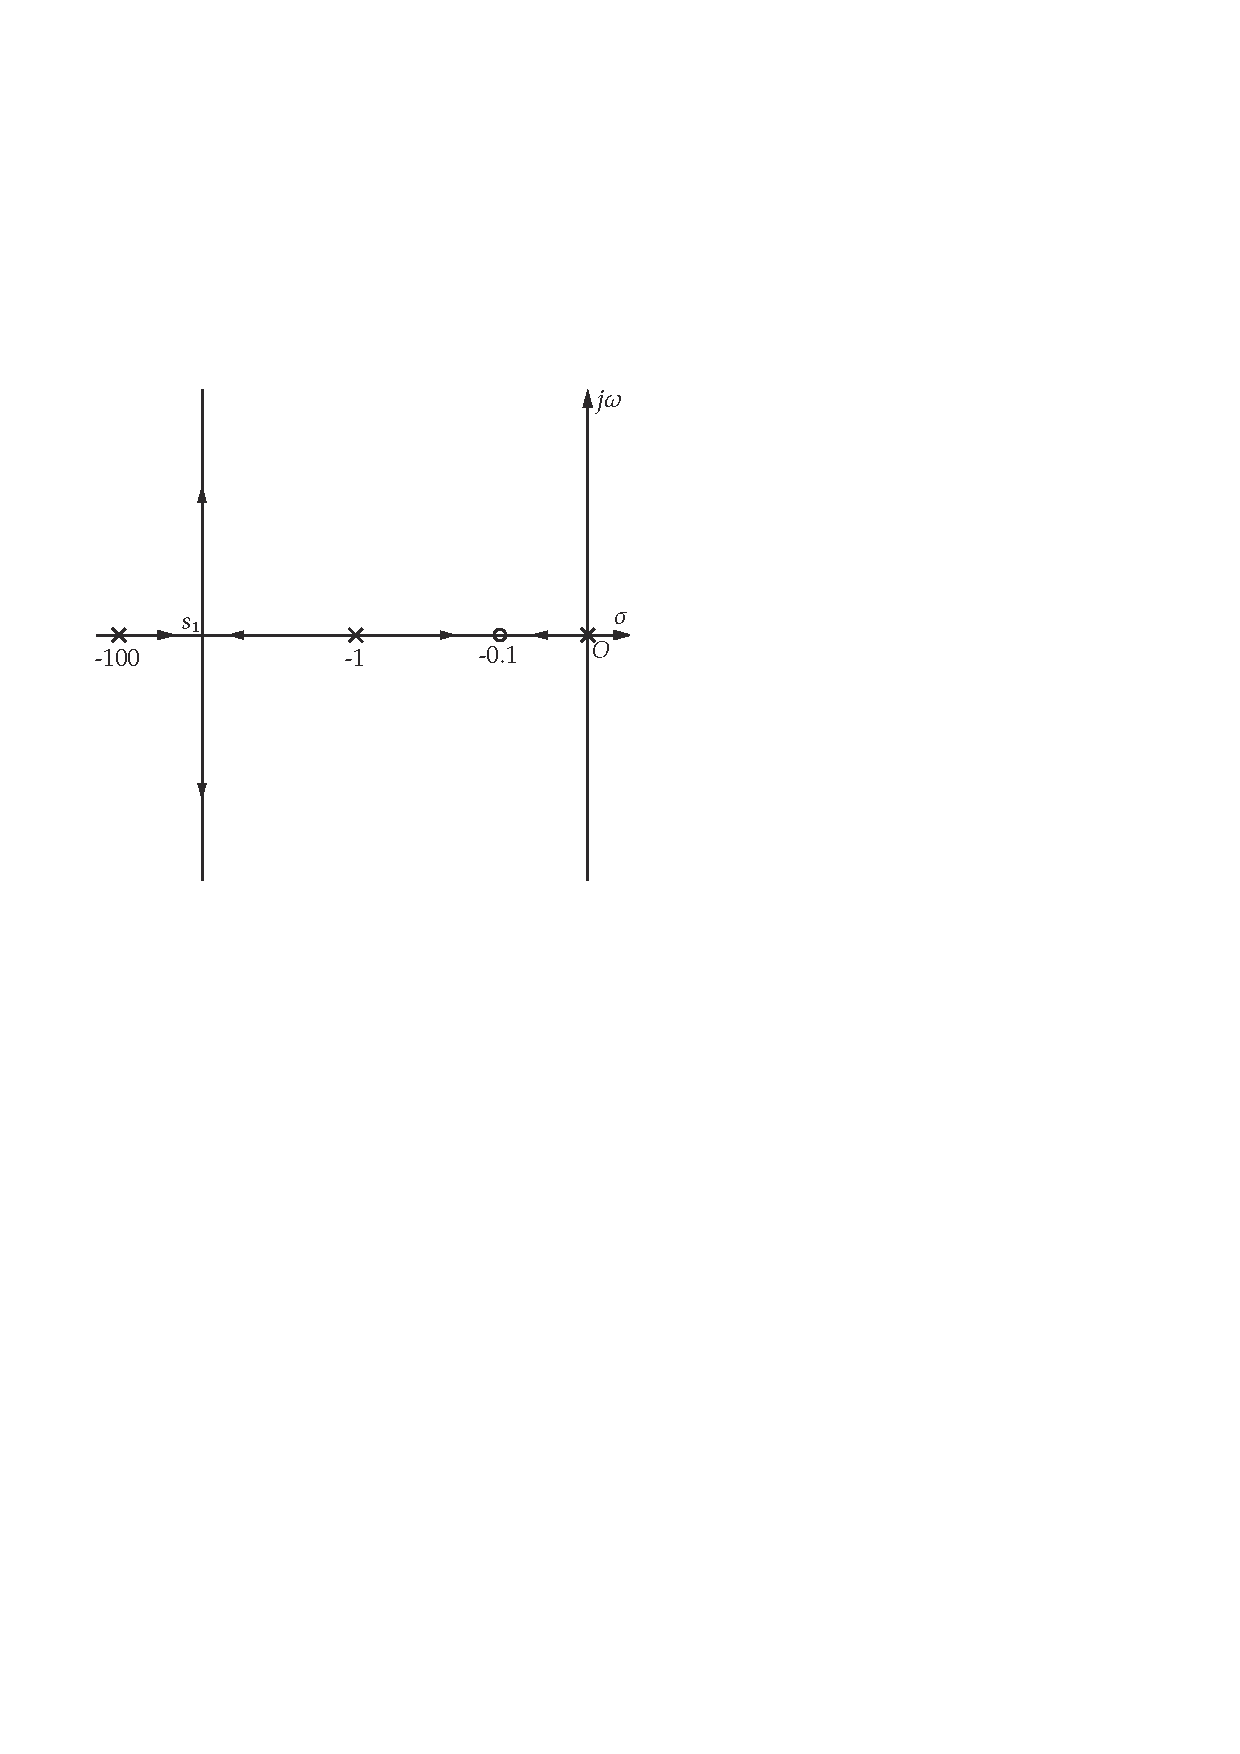
\includegraphics[scale=0.6]{figures/figure5.4.pdf}
        \end{figure}
    \end{enumerate}
\end{exercise}

\setcounter{exercise}{10}

\begin{exercise} % 5.11
    \begin{enumerate}
        \item 未考虑功率负反馈时
        \begin{equation*}
            \begin{cases}
                \dv{\Delta n}{t} = \frac{n_0}{\varLambda}\Delta \rho + \frac{\rho_0 - \beta}{\varLambda}\Delta n + \lambda \Delta c \\
                \dv{\Delta c}{t} = \frac{\beta}{\varLambda}\Delta n - \lambda \Delta c
            \end{cases}
        \end{equation*}
        \begin{equation*}
            \begin{bmatrix}
                \Delta \dot{n} \\
                \Delta \dot{c}
            \end{bmatrix} = \begin{bmatrix}
                -\frac{\beta}{\varLambda} & \lambda \\
                \frac{\beta}{\varLambda} & -\lambda
            \end{bmatrix} \begin{bmatrix}
                \Delta n \\
                \Delta c
            \end{bmatrix} + \begin{bmatrix}
                \frac{n_0}{\varLambda} \\
                0
            \end{bmatrix} \Delta \rho 
        \end{equation*}
        代入参量,得
        \begin{equation*}
            \symbfit{A} = \begin{bmatrix}
                -1.067 & 0.1 \\
                1.067 & -0.1
            \end{bmatrix}
        \end{equation*}
        李雅普诺夫函数$V(x) = x^{\top} \symbfit{P} x$,令$\symbfit{Q} = \symbfit{I}$,则$\symbfit{A}^{\top}\symbfit{P} + \symbfit{P}\symbfit{A} = -\symbfit{I}$,即
        \begin{equation*}
            \begin{bmatrix}
                -1.067 & 1.067 \\
                0.1 & -0.1
            \end{bmatrix} \begin{bmatrix}
                p_{11} & p_{12} \\
                p_{21} & p_{22}
            \end{bmatrix} + \begin{bmatrix}
                p_{11} & p_{12} \\
                p_{21} & p_{22}
            \end{bmatrix} \begin{bmatrix}
                -1.067 & 0.1 \\
                1.067 & -0.1
            \end{bmatrix} = \begin{bmatrix}
                -1 & 0 \\
                0 & 1
            \end{bmatrix}
        \end{equation*}
        解得
        \begin{equation*}
            \symbfit{P} = \begin{bmatrix}
                -2.009 & -2.478 \\
                -2.478 & -2.522
            \end{bmatrix}
        \end{equation*}
        该矩阵负定\footnote{该矩阵为手算的近似解,计算器可能显示无解,无论写哪个,只要说明了系统非大范围渐进稳定即可。},即系统在原点处平衡状态非大范围渐进稳定。
        \item 考虑功率负反馈时
        \begin{equation*}
            \begin{cases}
                \dv{\Delta n}{t} = \frac{n_0}{\varLambda}\Delta \rho + \frac{\rho_0 - \beta}{\varLambda}\Delta n + \lambda \Delta c \\
                \dv{\Delta c}{t} = \frac{\beta}{\varLambda}\Delta n - \lambda \Delta c \\
                \Delta \rho = \Delta \rho_{\rm ex} - \alpha_{\rm P} \Delta n
            \end{cases}
        \end{equation*}
        \begin{equation*}
            \begin{bmatrix}
                \Delta \dot{n} \\
                \Delta \dot{c}
            \end{bmatrix} = \begin{bmatrix}
                -\frac{\beta+n_0 \alpha_{\rm P}}{\varLambda} & \lambda \\
                \frac{\beta}{\varLambda} & -\lambda
            \end{bmatrix} \begin{bmatrix}
                \Delta n \\
                \Delta c
            \end{bmatrix} + \begin{bmatrix}
                \frac{n_0}{\varLambda} \\
                0
            \end{bmatrix} \Delta \rho_{\rm ex} 
        \end{equation*}
        同理,解得
        \begin{equation*}
            \symbfit{P} = \begin{bmatrix}
                303.8 & 307.9 \\
                307.9 & 312.9
            \end{bmatrix}
        \end{equation*}
        该矩阵正定,即系统在原点处平衡状态非大范围渐进稳定。
    \end{enumerate}
\end{exercise}